%%%%%%%%%%%%%%%%%%%%%%%%%%%%%%%%%%%%%%%%%%%%%%%%%%%%%%%%%%%%%%%%%%%%%%%%%%%%%%%
% Chapter 2: Desarrollo
%%%%%%%%%%%%%%%%%%%%%%%%%%%%%%%%%%%%%%%%%%%%%%%%%%%%%%%%%%%%%%%%%%%%%%%%%%%%%%%

%++++++++++++++++++++++++++++++++++++++++++++++++++++++++++++++++++++++++++++++
En este capítulo dos se va a describir el desarrollo del proyecto. Se dividirá en dos fases bien diferenciadas, una primera fase que consiste en el análisis y refactorización del código fuente de la versión anterior de
{\it GitHub Education Shell}, y una segunda fase que trata de la incorporación de nuevas funcionalidades a la herramienta.
\bigskip

Por otro lado, también cabe nombrar la metodología de trabajo empleada. Situándonos en el marco de las metodologías ágiles, {\it Scrum} fue la metodología que mejor encajaba, teniendo en cuenta las características del proyecto.
Se ha optado por un desarrollo incremental, en lugar de una planificación y ejecución estricta de las tareas. Además, en numerosas ocasiones,
se produjeron solapamientos de las diferentes partes del desarrollo, en vez de un ciclo secuencial. También fueron frecuentes las reuniones con el tutor, en las que se comentaban tanto avances como dificultades.

%++++++++++++++++++++++++++++++++++++++++++++++++++++++++++++++++++++++++++++++

\section{Primera fase: análisis}
\label{2:sec:1}

En esta sección, se explicará detalladamente el proceso fundamental de la primera fase de este Trabajo de Fin de Grado.
\bigskip
%---------------------------------------------------------------------------------
El análisis del código fuente correspondiente a la primera versión de {\it ghedsh}, se ha llevado a cabo con la finalidad de identificar aquellas partes mejorables del diseño e implementación,
puesto que una de las prioridades era facilitar el desarrollo colaborativo y, para ello, se requiere que el código sea limpio y fácil de entender, lo más auto-explicativo posible.
\bigskip

\subsubsection{Estructura del repositorio}
En la figura \ref{fig:masterv1}, se muestra la estructura del repositorio de la primera versión de {\it ghedsh}, en concreto, de la rama \verb master. Dicha estructura corresponde con la forma estándar
de organizar el código de las gemas.

\begin{figure}[H]
\begin{center}
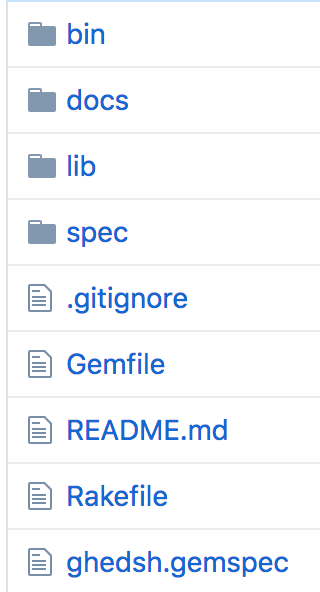
\includegraphics[width=0.20\textwidth]{images/estructura-inicial}
\caption{Estructura del repositorio (primera versión).}
\label{fig:masterv1}
\end{center}
\end{figure}

A continuación, se explicarán los componentes principales del repositorio:
\begin{itemize}
  \item {\it \textbf{bin}}: incluye el ejecutable de la gema, que se cargará en el \verb $PATH  del usuario.
  \item {\it \textbf{lib}}: en este directorio se encuentra el código fuente de la gema.
  \item {\it \textbf{spec}} o {\it \textbf{test}}: aquí se definirán las pruebas, que dependrán del {\it framework} de tests que utilice el desarrollador.
  \item {\it \textbf{Gemfile}}: es un fichero donde se especifican las dependencias del programa.
  \item {\it \textbf{Rakefile}}: se trata de un fichero muy común en las gemas. Su función es, principalmente, la automatización de tareas.
  \item {\it \textbf{gemspec}}: en este último fichero se incluye toda la información acerca de la gema, como, por ejemplo,
  su versión, plataforma soportada, versión de Ruby requerida y nombre y correo electrónico del autor o autores.
\end{itemize}
\bigskip

\subsubsection{Contenido del repositorio}
El primer paso del análisis consistió en comprender exactamente el flujo del programa. Ésto es necesario dado que, para identificar las partes mejorables del diseño inicial, requiere entenderlo en profundidad.
\bigskip

En la figura \ref{fig:lib}, vemos el contenido de \verb /lib :

\begin{figure}[H]
  \begin{center}
  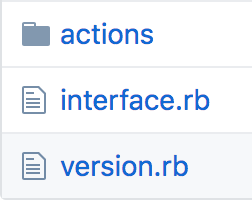
\includegraphics[width=0.25\textwidth]{images/lib}
  \caption{Contenido del directorio lib.}
  \label{fig:lib}
  \end{center}
\end{figure}

Los dos ficheros que ahí se encuentan son: \verb interface.rb  y \verb version.rb  .
\bigskip

En cuanto a \verb interface.rb , implementa la clase {\it Interface}. Ésta clase lleva a cabo el bucle principal característico de los CLI, se trata del bucle {\it Lectura-Evaluación-Impresión}
(en inglés, {\it REPL, Read-Eval-Print-Loop} \cite{B9}), que consiste en:
\begin{itemize}
  \item \textbf{Lectura}: parsea la entrada del usuario y determina si existe esa acción en la estructura de datos interna.
  \item \textbf{Evaluación}: una vez que se acepta la entrada del usuario se ejecutan las acciones con los parámetros especificados, si son necesarios. Es aquí donde se realiza el manejo de errores y excepciones.
  \item \textbf{Impresión}: muestra al usuario el resultado obtenido tras realizar el paso de evaluación.
\end{itemize}

Por otro lado, el fichero \verb version.rb , contiene una constante que indica la versión de la gema {\it ghedsh}. También cabe nombrar que, para asignar un identificador numérico a cada estado del software, se ha utilizado {\it Semantic Versioning} \cite{B10}.
\bigskip

A grandes rasgos, este esquema de control de versiones tiene la estructura {\it MAJOR.MINOR.PATCH}, donde
{\it MAJOR} se incrementa cuando se realizan cambios en la API que no son retrocompatibles. {\it MINOR} se modifica al añadir nuevas funcionalidades que sí son retrocompatibles y, por último, {\it PATCH} varía al corregir {\it bugs} en el software.
Un ejemplo de versión sería:
\begin{itemize}
  \item \verb ghedsh  \verb version  \verb 2.3.6 .
\end{itemize}
\bigskip

En cuanto al directorio \verb /lib/actions , la figura \ref{fig:actions} muestra el contenido del mismo:
\begin{figure}[H]
  \begin{center}
  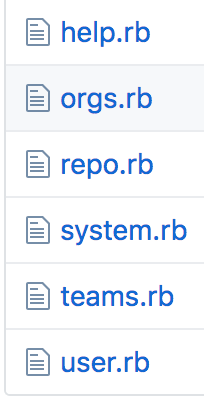
\includegraphics[width=0.17\textwidth]{images/actions}
  \caption{Contenido del directorio actions}
  \label{fig:actions}
  \end{center}
\end{figure}
\bigskip

Los ficheros principales se describirán según la funcionalidad que desempeñan:
\begin{itemize}
  \item \verb orgs.rb : proporciona los métodos necesarios relacionados con las organizaciones para comunicarse con la API de GitHub.
  \item \verb repo.rb : agrupa métodos que llevan a cabo tareas relacionadas con los repositorios, nuevamente, haciendo uso de la API de GitHub.
  \item \verb teams.rb : de manera similar a los anteriores ficheros, especializado en tareas de equipos.
  \item \verb user.rb : agrupa métodos relacionados con el usuario.
  \item \verb system.rb : este fichero se encarga de crear los directorios de configuración de {\it ghedsh}.
\end{itemize}
\bigskip

\subsubsection{Code Smell}
Una vez analizado el planteamiento inicial, se han detectado una serie de debilidades en el diseño que han dado lugar a diversos {\it code smell} \cite{B11}.
Un {\it code smell} se define como cualquier característica del código fuente que, posiblemente, indica un problema más profundo. No son considerados como {\it bugs}, puesto que no impiden que un programa funcione de manera correcta.
\bigskip

No obstante, estos defectos de diseño pueden afectar al rendimiento del programa, aumentan la probabilidad de errores en el futuro e, incluso, ralentizar el desarrollo del programa y dificultar la extensibilidad del mismo.
\bigskip

Determinar qué es y lo que no es un {\it code smell} para un código fuente específico suele tener un componente de juicio subjetivo, dado que puede variar según el lenguaje de programación utilizado, el desarrollador y la metodología de desarrollo aplicada. Pero, por otro lado, valorar 
los posibles casos de uso, aporta indicaciones para respetar ciertos principios y calidad del software.
\bigskip

En el apartado de refactorización se explicará cómo se ha procedido para solucionarlos. A continuación, se expondrán los {\it code smells} más significativos encontrados en la primera versión de {\it ghedsh}. 
\begin{itemize}
  \item \textbf{Switch Statements}: uno de los síntomas más comunes en código orientado a objetos.
\end{itemize}

  
%---------------------------------------------------------------------------------
\section{Segunda fase: refactorización}
\label{2:sec:2}
%---------------------------------------------------------------------------------
